\section{P, NP, Reductions}
\begin{itemize}
	\item Recall that P is a ``complexity class'' of problems that are efficiently solvable (by efficient, 
		we mean polynomial time), and NP being the complexity class of problems that can be verified 
		efficiently. (again, polynomial time)
	\item Examples of problems in NP are: 3-color problem, TSP, factoring integers.
\end{itemize}
\subsection{Rudrata Cycle (Hamiltonian cycle)}
\begin{itemize}
	\item Input: a graph \(G = (V, E)\), and we output a tour that visits each vertex exactly once. 
	\item We can just run through all \(n!\) cycles in the graph, which is highly inefficient. The best known 
		algorithm is \(O(1.657^n)\) (this is faster than the DP solution), so this is not a problem in P! 
	\item This problem is in NP, since given a string of vertices to visit, we can just go to our graph 
		and check. This can be done in polynomial time.  
	\item There are often modifications we can make to the problem that seemingly don't make that big of 
		a difference, but drastically simplify the problem: finding an Eulerian tour (which adds the constraint
		that every edge must be visited), for instance, is 
		a problem in \(P\). 
\end{itemize}

\subsection{Traveling Salesperson Problem (TSP)}
\begin{itemize}
	\item Input: a graph \(G = (V, E)\) with edge weight, and there are three variations to this problem:
		\begin{itemize}
			\item \textbf{Optimization TSP:} We're asked to find the tour with the minimum total weight. Our 
				DP solution gets a runtime to \(O(n^22^{n})\), but this isn't polynomial time, so this isn't in P.

				It's also not in NP, since there's no way to check whether a given tour is minimized 
				without knowing the weights of all other tours.
			\item \textbf{Search TSP:} Find a tour with total weight \(\le B\), where \(B\) denotes our
				``Budget''. This problem is not in P since coming up with a tour is still hard, but 
				it is in NP, since verifying that the budget is less than \(B\), can be done in polynomial time.  
				
				\comment{Notice that if we can solve Search TSP in polynomial time, this also gives a solution 
				to Optimization TSP in polynomial time!} 
			\item \textbf{Decision TSP:} Asks whether there exists a tour with weight \(\le B\). Again, just 
				like Search TSP, this problem is not in P but is in NP. 
		\end{itemize}
	\item There are a list of problems that are known to not be in NP. Examples are: some optimization version 
		of problems, counting problems (counting number of 3-colorings, for example), the halting problem.
	\item Formally, NP is only defined for \textbf{decision problems}. (CS172 material) For this class, 
		we'll be looser and allow search problems as well. 
\end{itemize}
\subsection{P vs. NP}
\begin{itemize}
	\item \textbf{Theorem:} \(\text P \subseteq \text{NP}\). In other words, any problem that can be 
		\textit{solved} in polynomial time can also be \textit{verified} in polynomial time. The verification 
		algorithm can literally just be to solve the problem again and check that the solutions match.
	\item A complexity diagram is usually used to show where problems lie:
		\begin{center}
			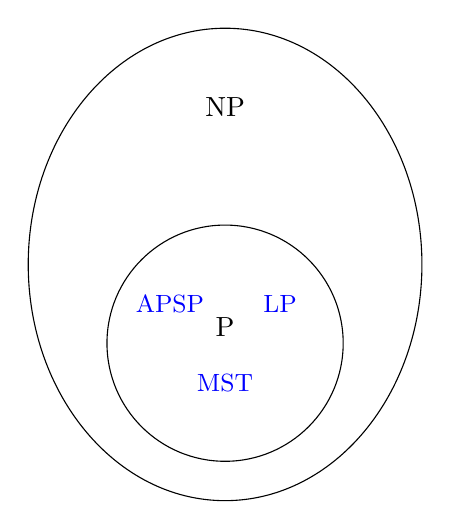
\begin{tikzpicture}
				\draw(0, 0) circle [radius=1.5cm];
				\draw node at (0, 0.2) {P};
				\draw (0, 1) ellipse [x radius = 2.5, y radius = 3];
				\draw node at (0, 3) {NP};
				\draw[blue] node at (0, -0.5) {\small MST};
				\draw[blue] node at (0.7, 0.5) {\small LP};
				\draw[blue] node at (-0.7, 0.5) {\small APSP};
			\end{tikzpicture}
		\end{center}
	\item Largest open problem in theoretical computer science: is P \(=\) NP? 
\end{itemize}
\subsection{Reductions}
\begin{itemize}
	\item We say that a problem A \textit{reduces in polynomial time} to problem B if you can use any efficient
		algorithm for B to efficiently solve A. Mathematically, we'd write this as 
		\[
		A \preceq_p B
		\] 
		Another way to say this is that ``A's difficulty is less than B's difficulty'', or that ``A is at most 
		as hard as B.''
\end{itemize}
\subsubsection{Zero Sum Games}
\begin{itemize}
	\item Recall the input: a payoff matrix \(M\), and we want to output the Row player's optimal 
		strategy.
	\item \textbf{Theorem:} zero sum games \(\preceq_p\) Linear programming
		\begin{itemize}
			\item In essence, we transfer the ZSG into a linear programming problem via a reduction 
				algorithm. Then, take the LP input and run the LP algortihm on it (which is polynomial time),
				then run a recovery algorithm to go from the LP back to the ZSG. 
			\item As a general picture, we have 
				\begin{center}
					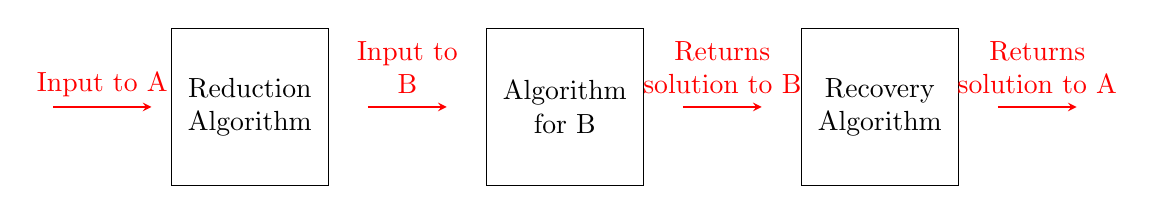
\begin{tikzpicture}[every text node part/.style={align=center}]
						\draw [-stealth, red]  (-1.5, 1) -- node[midway, above] {Input to A} (-0.25, 1);
						\foreach \x in {0, 4, 8} 
						\draw (\x, 0) -- (\x+2,0) -- (\x+2, 2) -- (\x, 2) -- cycle;
						\foreach \x in {2, 6, 10}
						\draw[-stealth, red] (\x+0.5, 1) -- (\x+1.5, 1);
						\draw node at (1, 1) {Reduction \\ Algorithm};	
						\draw node at (5, 1) {Algorithm \\ for B};
						\draw node at (9, 1) {Recovery \\ Algorithm};
						\draw[red] node at (3, 1.5) {Input to \\ B};
						\draw[red] node at (7, 1.5) {Returns \\ solution to B};
						\draw[red] node at (11, 1.5) {Returns \\ solution to A};
					\end{tikzpicture}
				\end{center}
		\end{itemize}
\end{itemize}
\subsubsection{Rudrata Cycle vs. Min TSP}
\begin{itemize}
	\item It can also be shown that finding a Rudrata cycle reduces to the min-TSP problem, since both problems 
		require us to find tours, then finding a Rudrata cycle is at most as hard as min-TSP.  
	\item This is because finding a Hamiltonian tour is effectively finding a cycle on this graph that visits
		all vertices, which is exactly what min-TSP is doing except with more restrictions.
\end{itemize}
